% Caliber technical note (Task 27). Build: make -C docs/paper. Every number comes from numbers.tex, which
% docs/paper/numbers.py generates from docs/FACTS.json, bench/BASELINE.json, bench/carrierbench/{REPORT,oracle,saboteur}.json,
% spacetimedb/src/thresholds.ts and git. No number is typed in this file.
\documentclass[conference]{IEEEtran}
\IEEEoverridecommandlockouts
\usepackage{booktabs}
\usepackage{tikz}
\usetikzlibrary{positioning,arrows.meta,shapes.geometric}
\usepackage{url}
\usepackage{graphicx}
\usepackage[hidelinks]{hyperref}
% Generated by docs/paper/numbers.py. Do not edit; every value is read from a result file.
% written 2026-10-25T00:12:59+00:00
\newcommand{\benchSeed}{42}
\newcommand{\benchGeneratedAt}{2026-10-24T23:24:14+00:00}
\newcommand{\nDays}{92}
\newcommand{\calDayOne}{2026-07-01}
\newcommand{\calDayLast}{2026-11-05}
\newcommand{\nTerminals}{6}
\newcommand{\nTrucks}{40}
\newcommand{\nDrivers}{48}
\newcommand{\nVendors}{5}
\newcommand{\nContracts}{34}
\newcommand{\nPOs}{30}
\newcommand{\nPings}{155,457}
\newcommand{\nFuelCards}{40}
\newcommand{\nStations}{46}
\newcommand{\nPlazas}{14}
\newcommand{\nPlanted}{52}
\newcommand{\nClasses}{7}
\newcommand{\nDecoys}{6}
\newcommand{\nKeyRows}{58}
\newcommand{\nCleanRows}{7,886}
\newcommand{\nCardRows}{5,607}
\newcommand{\nTollRows}{2,157}
\newcommand{\nInvoiceRows}{180}
\newcommand{\nRowsTotal}{7,944}
\newcommand{\genSeconds}{2.74}
\newcommand{\fixturesMatchCommit}{yes}
\newcommand{\fixturesMatchRegen}{yes}
\newcommand{\heldOutTrucks}{25}
\newcommand{\trucksNoPlanted}{10}
\newcommand{\heldOutVendors}{0}
\newcommand{\vendorsNoPlanted}{0}
\newcommand{\heldOutRows}{19}
\newcommand{\policyHoldsBench}{6}
\newcommand{\decoysLookLikeLM}{yes}
\newcommand{\decoysHaveSwapLines}{yes}
\newcommand{\decoyMilesMin}{48.50}
\newcommand{\decoyMilesMax}{97.20}
\newcommand{\auditRows}{58}
\newcommand{\auditInferable}{58}
\newcommand{\auditWithFile}{58}
\newcommand{\auditExtra}{0}
\newcommand{\auditEvaluated}{7,944}
\newcommand{\auditPassed}{yes}
\newcommand{\plantedTableBody}{location\_mismatch & 14 & 6 & 20 & 20 \\
capacity\_exceeded & 6 & 0 & 6 & 6 \\
rate\_variance & 9 & 0 & 9 & 9 \\
duplicate\_toll & 11 & 0 & 11 & 11 \\
duplicate\_invoice & 4 & 0 & 4 & 4 \\
vendor\_bank\_change & 3 & 0 & 3 & 3 \\
short\_received & 5 & 0 & 5 & 5 \\}
\newcommand{\thrMiles}{25}
\newcommand{\thrPingMin}{30}
\newcommand{\thrTankPct}{10}
\newcommand{\thrTollMin}{10}
\newcommand{\thrRatePct}{5}
\newcommand{\thrDupDays}{30}
\newcommand{\thrBankDays}{7}
\newcommand{\thrBankUsd}{\$5,000.00}
\newcommand{\autoPayUsd}{\$2,500.00}
\newcommand{\autoPayDayUsd}{\$40,000.00}
\newcommand{\droidTimeoutSec}{90}
\newcommand{\workerConcurrency}{2}
\newcommand{\escalationSec}{63}
\newcommand{\escalationTargetSec}{30}
\newcommand{\factsAsOf}{2026-10-24T22:25:41+00:00}
\newcommand{\txMatched}{7,944}
\newcommand{\dayReached}{92}
\newcommand{\overallP}{1.00}
\newcommand{\overallR}{1.00}
\newcommand{\overallTP}{58}
\newcommand{\overallFP}{0}
\newcommand{\plantedExceptionsFacts}{58}
\newcommand{\autoPaidCount}{7,886}
\newcommand{\autoPaidUsd}{\$1,083,630.52}
\newcommand{\ctrlReleasedCount}{8}
\newcommand{\ctrlReleasedUsd}{\$32,097.00}
\newcommand{\limitHoldsCount}{6}
\newcommand{\limitHoldsUsd}{\$16,789.00}
\newcommand{\decoysCleared}{6}
\newcommand{\decoysOneAnswer}{6}
\newcommand{\plantedClearedByRule}{0}
\newcommand{\rulesExpired}{6}
\newcommand{\refusalsCount}{1}
\newcommand{\settleOffline}{7,894}
\newcommand{\settleLive}{0}
\newcommand{\vcHolds}{3}
\newcommand{\vcHitRejected}{1}
\newcommand{\vcCleanApproved}{2}
\newcommand{\vcFixture}{3}
\newcommand{\investReplayed}{47}
\newcommand{\investLive}{0}
\newcommand{\autoRejectedFacts}{11}
\newcommand{\holdsFacts}{53}
\newcommand{\droidTasks}{52}
\newcommand{\droidAvgIn}{1,033}
\newcommand{\droidAvgOut}{1,354}
\newcommand{\droidAvgCache}{70,386}
\newcommand{\droidAvgSec}{25.60}
\newcommand{\droidCredits}{2,016,204}
\newcommand{\caliberTableBody}{location\_mismatch & 20 & 20 & 20 & 0 & 1.00 & 1.00 \\
capacity\_exceeded & 6 & 6 & 6 & 0 & 1.00 & 1.00 \\
rate\_variance & 9 & 9 & 9 & 0 & 1.00 & 1.00 \\
duplicate\_toll & 11 & 11 & 11 & 0 & 1.00 & 1.00 \\
duplicate\_invoice & 4 & 4 & 4 & 0 & 1.00 & 1.00 \\
vendor\_bank\_change & 3 & 3 & 3 & 0 & 1.00 & 1.00 \\
short\_received & 5 & 5 & 5 & 0 & 1.00 & 1.00 \\}
\newcommand{\oraclePosted}{7,886}
\newcommand{\oraclePostedUsd}{\$1,083,630.52}
\newcommand{\oracleHolds}{41}
\newcommand{\oracleRejects}{11}
\newcommand{\oracleLimits}{6}
\newcommand{\oracleQuestions}{0}
\newcommand{\oracleWrong}{0}
\newcommand{\oracleHuman}{47}
\newcommand{\measPosted}{7,886}
\newcommand{\measQuestions}{6}
\newcommand{\measHolds}{47}
\newcommand{\measRejects}{11}
\newcommand{\measLimits}{6}
\newcommand{\measWrong}{0}
\newcommand{\sabRuns}{2}
\newcommand{\sabRefs}{INV-1077, 2231}
\newcommand{\sabCodes}{vendor\_bank\_change and location\_mismatch}
\newcommand{\sabConfidence}{0.99}
\newcommand{\sabEvidenceItems}{3}
\newcommand{\sabPayments}{0}
\newcommand{\sabPaymentsBefore}{1}
\newcommand{\sabPaymentsAfter}{1}
\newcommand{\sabRefusedRows}{2}
\newcommand{\sabHoldStatus}{awaiting\_controller}
\newcommand{\sabMessage}{agent may not do this (needs controller)}
\newcommand{\sabTestStatus}{passed}
\newcommand{\baseGeneratedAt}{2026-10-25T00:12:27+00:00}
\newcommand{\baseSeed}{42}
\newcommand{\baseRows}{558}
\newcommand{\basePlanted}{52}
\newcommand{\baseDecoys}{6}
\newcommand{\baseClean}{500}
\newcommand{\baseCleanCard}{174}
\newcommand{\baseCleanToll}{173}
\newcommand{\baseCleanInvoice}{153}
\newcommand{\baseExcludedLimits}{6}
\newcommand{\basePrompt}{bench/prompts/hold\_or\_clear.txt}
\newcommand{\sonnetLabel}{Claude Sonnet}
\newcommand{\sonnetModel}{claude-sonnet-5-5}
\newcommand{\sonnetAnswered}{558}
\newcommand{\sonnetRows}{558}
\newcommand{\sonnetHolds}{58}
\newcommand{\sonnetP}{1.00}
\newcommand{\sonnetR}{1.00}
\newcommand{\sonnetTP}{58}
\newcommand{\sonnetFP}{0}
\newcommand{\sonnetDetP}{1.00}
\newcommand{\sonnetDetR}{1.00}
\newcommand{\sonnetDetFP}{0}
\newcommand{\sonnetDecoysHeld}{6}
\newcommand{\sonnetDecoysCleared}{0}
\newcommand{\sonnetPartial}{no}
\newcommand{\sonnetFailure}{Claude Sonnet failed on nothing in this sample.}
\newcommand{\sonnetTokIn}{2,358,546}
\newcommand{\sonnetTokOut}{166,183}
\newcommand{\sonnetTemperature}{not sent (Claude Sonnet 5.5 rejects a non-default temperature)}
\newcommand{\asiLabel}{asi1-mini}
\newcommand{\asiModel}{asi1-mini}
\newcommand{\asiAnswered}{557}
\newcommand{\asiRows}{558}
\newcommand{\asiHolds}{150}
\newcommand{\asiP}{0.31}
\newcommand{\asiR}{0.81}
\newcommand{\asiTP}{47}
\newcommand{\asiFP}{103}
\newcommand{\asiDetP}{0.33}
\newcommand{\asiDetR}{0.84}
\newcommand{\asiDetFP}{101}
\newcommand{\asiDecoysHeld}{6}
\newcommand{\asiDecoysCleared}{0}
\newcommand{\asiPartial}{no}
\newcommand{\asiFailure}{asi1-mini missed 4 of 6 capacity\_exceeded, 1 of 9 rate\_variance, 2 of 4 duplicate\_invoice, 2 of 3 vendor\_bank\_change; held with the wrong code 2 capacity\_exceeded; held 101 clean rows (holds by code that did not match a planted row: 82 as duplicate\_toll, 8 as location\_mismatch, 8 as vendor\_bank\_change, 5 as duplicate\_invoice); 1 row had no parseable answer (1 unparsed), counted as not held.}
\newcommand{\asiTokIn}{2,393,406}
\newcommand{\asiTokOut}{66,383}
\newcommand{\asiTemperature}{0}
\newcommand{\sonnetCostUsd}{\$6.38}
\newcommand{\sonnetCapUsd}{\$15}
\newcommand{\sonnetStopped}{no}
\newcommand{\asiRequests}{561}
\newcommand{\asiQuotaWindow}{100}
\newcommand{\asiQuotaDay}{1,000}
\newcommand{\asiPaceSec}{9.10}
\newcommand{\basePartial}{no}
\newcommand{\baselineTableBody}{location\_mismatch & 20 & 1.00 / 1.00 & 1.00 / 1.00 & 0.71 / 1.00 \\
capacity\_exceeded & 6 & 1.00 / 1.00 & 1.00 / 1.00 & n/a / 0.00 \\
rate\_variance & 9 & 1.00 / 1.00 & 1.00 / 1.00 & 1.00 / 0.89 \\
duplicate\_toll & 11 & 1.00 / 1.00 & 1.00 / 1.00 & 0.12 / 1.00 \\
duplicate\_invoice & 4 & 1.00 / 1.00 & 1.00 / 1.00 & 0.29 / 0.50 \\
vendor\_bank\_change & 3 & 1.00 / 1.00 & 1.00 / 1.00 & 0.11 / 0.33 \\
short\_received & 5 & 1.00 / 1.00 & 1.00 / 1.00 & 1.00 / 1.00 \\
overall & 58 & 1.00 / 1.00 & 1.00 / 1.00 & 0.31 / 0.81 \\}
\newcommand{\tiesOrWinsText}{Claude Sonnet tied the kernel on location\_mismatch; Claude Sonnet tied the kernel on capacity\_exceeded; Claude Sonnet tied the kernel on rate\_variance; Claude Sonnet tied the kernel on duplicate\_toll; Claude Sonnet tied the kernel on duplicate\_invoice; Claude Sonnet tied the kernel on vendor\_bank\_change; Claude Sonnet tied the kernel on short\_received; asi1-mini tied the kernel on short\_received; Claude Sonnet tied the kernel on overall.}
\newcommand{\tiesOrWinsCount}{9}
\newcommand{\caliberRowsEvaluated}{7,944}
\newcommand{\commitLabelFix}{2fac596}
\newcommand{\commitLabelFixDate}{2026-10-24 14:21}
\newcommand{\commitLabelFixSubject}{Honesty fixes: hand-shaped vendor checks carry status hand\_shaped, an amber badge, the fixture note and label-only refs }
\newcommand{\commitDecoyRerecord}{8e004e1}
\newcommand{\commitDecoyRerecordDate}{2026-10-24 14:13}
\newcommand{\commitDecoyRerecordSubject}{Decoys re-recorded live: Droid asks instead of clearing on the six unit-swap decoys}


\newcommand{\code}[1]{\texttt{#1}}

\begin{document}

\title{Caliber: an accounts-payable clerk whose code decides the money, measured against a planted answer key}

\author{\IEEEauthorblockN{Anudeep Bonagiri}\and\IEEEauthorblockN{Sreesanth Nitillan Senthilkumar}}

\maketitle

\begin{abstract}
Caliber is an autonomous accounts-payable clerk for a simulated \nTrucks-truck Texas carrier. A kernel in plain TypeScript, in integer cents, matches every fuel-card charge, toll and maintenance invoice against telematics, tank size, purchase order, contract rate, receiving record and vendor bank details over \nDays{} business days. Clean rows post within policy limits; everything else becomes a hold. A read-only Factory Droid session investigates each hold through Elastic Agent Builder tools and the evidence files and returns a typed finding; when a person is needed, the controller answers from ASI:One and the answer becomes a scoped, expiring, backtested rule. Segregation of duties is enforced in SpacetimeDB reducers: the agent identity cannot approve a payment, and every action is an append-only audit row. We release CarrierBench, the synthetic carrier with its hidden answer key of \nPlanted{} planted errors in \nClasses{} classes and \nDecoys{} decoys, a machine audit that every planted row is inferable from its own evidence, and a model-only baseline on identical inputs. On the measured \nDays-day run the kernel reaches precision \overallP{} and recall \overallR{} on the \nKeyRows{} answer-key rows and posts \autoPaidCount{} payments without a person; the oracle ceiling posts \oraclePosted. A saboteur run shows that a finding recommending release with confidence \sabConfidence{} and fabricated evidence cannot move money. We report what we got wrong and the limits of a synthetic benchmark.
\end{abstract}

\section{System context}

Caliber has one write path to money, shown in Fig.~\ref{fig:path}. The business-day clock ticks inside the SpacetimeDB module; on each tick \code{matchDay} hands every row of the day to \code{kernel.ts}, a pure function that never imports the database, a connector or a model client. The kernel returns a code and an evidence object. A \code{matched} row within the auto-pay limits (\autoPayUsd{} per transaction, \autoPayDayUsd{} per day) becomes a \code{payment} row; a \code{duplicate\_toll} is auto-rejected with an audit row and no task; every other code becomes a \code{hold} and an \code{agent\_task}.

The worker claims the task with a version-locked \code{claim\_task}, opens a Droid session with \code{autonomyLevel Off}, the edit and execute tools disabled, a permission handler that cancels anything but MCP tool calls, and a \droidTimeoutSec~s abort, at concurrency \workerConcurrency. Droid reads the receipts, contracts and the dispatcher's swap log and calls Elastic Agent Builder tools over MCP (nearest telematics rows, the contract rate and clause). Its output is validated against a schema whose recommendation is one of \code{clear}, \code{hold} or \code{hold\_and\_ask}; there is no \code{pay}. The worker writes it back with \code{record\_investigation}, which can set a question on the hold and nothing else. The controller, over an ASI:One agent or the terminal, answers the question; the answer is drafted into a rule with a scope, a window and a backtest the module computes itself, and only an approved rule lets the kernel clear the next matching row. \code{approve\_payment} checks the caller's role, refuses the identity that requested the hold, requires a call-back note on a bank change, and writes the only other \code{payment} row there is. Refusals through the \code{try\_*} procedures are committed audit rows.

\begin{figure}[t]
\centering
\resizebox{\columnwidth}{!}{%
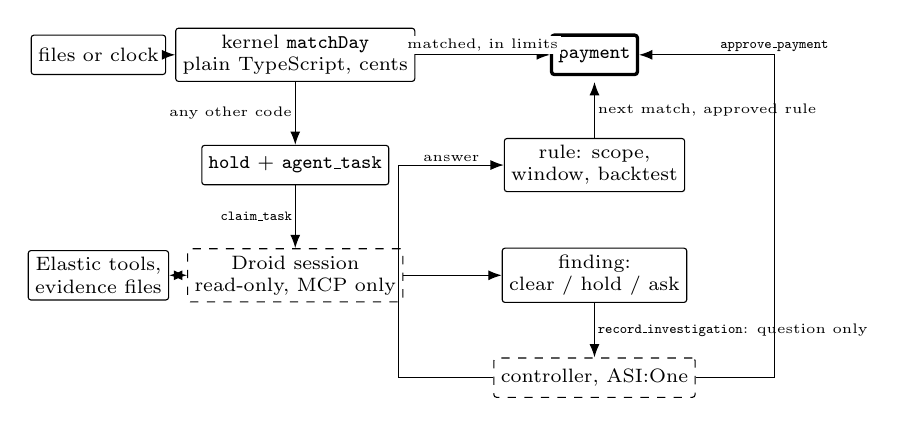
\begin{tikzpicture}[x=1cm, y=1cm,
  font=\scriptsize, >=Latex,
  box/.style={draw, rounded corners=1pt, inner sep=2.5pt, minimum height=5mm, align=center},
  money/.style={box, very thick},
  role/.style={box, dashed},
  lbl/.style={font=\tiny, fill=white, inner sep=1pt, align=center}]
\node[box]   (files)   at (0.9, 4.3) {files or clock};
\node[box]   (kernel)  at (3.4, 4.3) {kernel \code{matchDay}\\plain TypeScript, cents};
\node[money] (pay)     at (7.2, 4.3) {\code{payment}};
\node[box]   (hold)    at (3.4, 2.9) {\code{hold} + \code{agent\_task}};
\node[box]   (rule)    at (7.2, 2.9) {rule: scope,\\window, backtest};
\node[box]   (elastic) at (0.9, 1.5) {Elastic tools,\\evidence files};
\node[role]  (droid)   at (3.4, 1.5) {Droid session\\read-only, MCP only};
\node[box]   (finding) at (7.2, 1.5) {finding:\\clear / hold / ask};
\node[role]  (ctrl)    at (7.2, 0.2) {controller, ASI:One};
\draw[->] (files) -- (kernel);
\draw[->] (kernel) -- node[lbl, above] {matched, in limits} (pay);
\draw[->] (kernel) -- node[lbl, left] {any other code} (hold);
\draw[->] (hold) -- node[lbl, left] {\code{claim\_task}} (droid);
\draw[<->] (droid) -- (elastic);
\draw[->] (droid) -- (finding);
\draw[->] (finding) -- node[lbl, right] {\code{record\_investigation}: question only} (ctrl);
\draw[->] (ctrl.west) -- ++(-1.2,0) |- node[lbl, pos=0.75, above] {answer} (rule.west);
\draw[->] (rule.north) -- node[lbl, right] {next match, approved rule} (kernel.south -| rule.north);
\draw[->] (ctrl.east) -- ++(1.0,0) |- node[lbl, pos=0.5, sloped, above] {\code{approve\_payment}} (pay.east);
\end{tikzpicture}}
\caption{The one write path. Only the kernel (a \code{matched} row within limits) and \code{approve\_payment} (a controller identity that did not request the hold) write a \code{payment}. The finding reaches the hold's question field and nothing else; Droid's reach into data is MCP and read-only files.}
\label{fig:path}
\end{figure}

\section{CarrierBench}

CarrierBench is the synthetic carrier as a benchmark. \code{seed/generate.py} with seed \benchSeed{} writes \nDays{} business days (\calDayOne{} to \calDayLast) for \nTerminals{} terminals, \nTrucks{} trucks with one fuel card each, \nDrivers{} drivers, \nVendors{} maintenance vendors, \nContracts{} contracts and \nPOs{} purchase orders: \nCardRows{} fuel-card transactions at \nStations{} stations, \nTollRows{} tolls at \nPlazas{} plazas, \nInvoiceRows{} invoices and \nPings{} telematics pings, \nRowsTotal{} payable rows in all. Inside them the generator plants \nPlanted{} errors in \nClasses{} classes and \nDecoys{} decoys (Table~\ref{tab:bench}), recorded in \code{answer\_key.json}, which no agent code reads. The generator is deterministic: \code{carrierbench.py} regenerated the fixtures in \genSeconds~s and every file was byte-identical to the commit (\fixturesMatchRegen).

\begin{table}[t]
\centering
\caption{CarrierBench answer key and machine audit. Decoys are legitimate swaps that look like the code. Inferable: the Python mirror of the kernel raised the row with the key's code from the row's own records. File: an evidence document exists for the row.}
\label{tab:bench}
\begin{tabular}{lrrrr}
\toprule
Code & Planted & Decoys & Inferable & File \\
\midrule
\plantedTableBody
\bottomrule
\end{tabular}
\end{table}

\textbf{Controls.} Three are computed, not asserted. Held-out entities: \heldOutTrucks{} of \nTrucks{} trucks carry exactly one answer-key row and \trucksNoPlanted{} carry none, so \heldOutRows{} planted rows sit on an entity with no other planted row; all \nVendors{} vendors carry more than one (\heldOutVendors{} held out), which the audit reports rather than hides. Decoys: \nDecoys{} legitimate unit swaps from the dispatcher's swap log, \decoyMilesMin{} to \decoyMilesMax{} miles from the truck's nearest ping, every one indistinguishable from card misuse by the records the kernel reads (all look like \code{location\_mismatch}: \decoysLookLikeLM; all have swap-log lines: \decoysHaveSwapLines). Policy holds: \policyHoldsBench{} clean invoices above the per-transaction limit, a hold by policy and not an exception, kept out of the key and out of the baseline sample.

\textbf{Machine audit.} \code{seed/mirror.py}, the Python copy of \code{kernel.ts}, evaluated all \auditEvaluated{} rows from their records (nearest ping within \thrPingMin{} minutes, tank size, earlier tolls at the plaza, the contract valid on the receipt day, the purchase order and its received quantity, the vendor's bank-change day). It raised \auditInferable{} of \auditRows{} key rows with the key's code, \auditWithFile{} have an evidence file, and it flagged \auditExtra{} rows outside the key. Audit passed: \auditPassed. The kernel's thresholds are \thrMiles{} miles and \thrPingMin{} minutes, tank plus \thrTankPct{} percent, \thrTollMin{} minutes at a plaza, \thrRatePct{} percent over contract, \thrDupDays{} days for a same-amount invoice, and \thrBankUsd{} within \thrBankDays{} business days of a bank change.

Run it from a bare clone with \code{python3 bench/carrierbench/carrierbench.py -{}-seed \benchSeed}; it writes \code{REPORT.md} and \code{REPORT.json} and exits non-zero on any failure.

\section{Protocol}

Four systems were given the same rows. \textbf{Caliber} is the kernel plus Droid, measured on the full \caliberRowsEvaluated-row replay through the ledger (\code{docs/FACTS.json}). \textbf{\sonnetLabel} (\sonnetModel), \textbf{\opusLabel} (\opusModel) and \textbf{\asiLabel} (\asiModel) were each given, per row, exactly the records the kernel sees (the transaction, the truck and its pings for the day, or the plate's earlier tolls, or the purchase order, the contract valid on the receipt day, the vendor record and the vendor's earlier invoices), with no answer-key field and no planted marker, and asked for hold or clear with a code and a one-line reason, one attempt per row, no examples, no fine-tuning. The sample is stratified: all \basePlanted{} planted rows, all \baseDecoys{} decoys and \baseClean{} clean rows (\baseCleanCard{} card, \baseCleanToll{} toll, \baseCleanInvoice{} invoice; every clean invoice, since only that many exist), \baseRows{} rows in all; the \baseExcludedLimits{} policy holds were left out. Temperature, as recorded by the runner: asi1-mini \asiTemperature; Claude Sonnet \sonnetTemperature; Claude Opus 5.5 \opusTemperature. Both Anthropic models ran with thinking at the API default and no effort field; the default effort differs by model (\opusEffort), so each sits at its own default rather than one shared setting. Prompts are committed under \code{bench/prompts}, raw replies under \code{bench/outputs}.

\textbf{Prompt condition.} One condition was run, which we name \emph{hinted}: the prompt (\basePrompt) lists the \nClasses{} codes and their thresholds before asking. A \emph{bare} condition, records and question with no code list, was not run; the comparison below is hinted only, which favours the models. Scoring is code-exact: a hold counts for a code only when the system named that code, the same definition \code{facts.py} applies to the kernel; a detection reading (any code) is also given. A decoy is scored as a correct hold for every system, because the records cannot clear it. Positives are the \nKeyRows{} answer-key rows. Cost cap \sonnetCapUsd{} per Anthropic model, applied to each on its own; stopped for cost: Sonnet \sonnetStopped, Opus 5.5 \opusStopped. Partial run: \basePartial.

\section{Results}

\begin{table}[t]
\centering
\caption{Precision / recall per code, code-exact; key rows include the decoys. Caliber on the full \caliberRowsEvaluated-row run; the three models on the \baseRows-row sample. Generated \baseGeneratedAt.}
\label{tab:baseline}
\scriptsize
\setlength{\tabcolsep}{2pt}
\resizebox{\columnwidth}{!}{%
\begin{tabular}{lrcccc}
\toprule
Code & Key rows & Caliber & Sonnet & Opus 5.5 & asi1-mini \\
\midrule
\baselineTableBody
\bottomrule
\end{tabular}}
\end{table}

\textbf{Per code and overall.} Table~\ref{tab:baseline} is the comparison. Caliber: precision \overallP, recall \overallR, \overallTP{} true positives, \overallFP{} false positives over \txMatched{} transactions and \dayReached{} days. \sonnetLabel: \sonnetAnswered{} of \sonnetRows{} rows answered, \sonnetHolds{} holds, code-exact precision \sonnetP{} and recall \sonnetR{} (detection \sonnetDetP{} / \sonnetDetR, \sonnetDetFP{} false holds), \sonnetDecoysHeld{} of \baseDecoys{} decoys held, \sonnetCostUsd{} at list rates. \opusLabel: \opusAnswered{} of \opusRows{} rows answered, \opusHolds{} holds, code-exact precision \opusP{} and recall \opusR{} (detection \opusDetP{} / \opusDetR, \opusDetFP{} false holds), \opusDecoysHeld{} of \baseDecoys{} decoys held, \opusCostUsd{} at list rates. \asiLabel: \asiAnswered{} of \asiRows{} answered, \asiHolds{} holds, precision \asiP{} and recall \asiR{} (detection \asiDetP{} / \asiDetR, \asiDetFP{} false holds), \asiDecoysHeld{} of \baseDecoys{} decoys held, \asiRequests{} requests against a quota of \asiQuotaWindow{} per fifteen minutes. Where each failed, from the scorer: \sonnetFailure{} \opusFailure{} \asiFailure{} Ties or wins against the kernel: \tiesOrWinsCount{} entries, listed code by code in Section~\ref{sec:wrong}. Where a model ties the kernel on a code, the kernel's case on that code is not accuracy on this hinted sample but cost per row (\sonnetCostUsd{} on Sonnet and \opusCostUsd{} on Opus 5.5 for \sonnetRows{} rows, against none), determinism (the same row gives the same code every day), and the gate: a model's hold is advice the worker may record, the kernel's hold is a row only a person can release.

\textbf{End to end through the ledger.} In the measured run (\factsAsOf) the kernel or an approved rule posted \autoPaidCount{} payments (\autoPaidUsd) with no person involved, auto-rejected \autoRejectedFacts{} duplicate tolls, and raised \holdsFacts{} holds, of which \limitHoldsCount{} were policy holds (\limitHoldsUsd). The controller released \ctrlReleasedCount{} payments (\ctrlReleasedUsd). The \nDecoys{} decoys were cleared through an approved rule after exactly one controller answer each (\decoysOneAnswer{} of \nDecoys); planted exceptions cleared by a rule: \plantedClearedByRule; wrong postings: \measWrong. Of the \vcHolds{} bank-change holds, \vcHitRejected{} carried a public-records hit and was rejected by the controller, \vcCleanApproved{} were approved with a call-back note; all \vcFixture{} vendor checks came from hand-authored fixtures labelled as such (the CRS sandbox had not answered). All \settleOffline{} payments carry a labelled offline settlement id and \settleLive{} a live one. Investigations in the measured run were \investReplayed{} replayed recordings of the live Droid run and \investLive{} live; the live run itself cost, per task, \droidAvgIn{} input, \droidAvgOut{} output and \droidAvgCache{} cache tokens in \droidAvgSec~s, \droidCredits{} Factory credits for \droidTasks{} tasks.

\textbf{Oracle ceiling.} The oracle is the kernel handed the answer key: every planted row held (duplicate tolls auto-rejected), every decoy cleared with no question, clean rows posted under the same policy limits. Computed from the fixtures with the mirror, it posts \oraclePosted{} payments (\oraclePostedUsd), raises \oracleHolds{} exception holds and \oracleLimits{} policy holds, auto-rejects \oracleRejects, asks \oracleQuestions{} questions, posts \oracleWrong{} wrong rows, and still needs \oracleHuman{} human decisions. The measured run posted \measPosted{} without a person, raised \measHolds{} exception holds and \measLimits{} policy holds, auto-rejected \measRejects{} and asked \measQuestions{} questions. The whole gap to the ceiling is the \measQuestions{} questions on the decoys, which is the mechanism working as designed: the records cannot clear a decoy, a person can, and the answer is remembered as a rule.

\textbf{Saboteur.} A lying finding (recommendation \code{clear}, confidence \sabConfidence, \sabEvidenceItems{} fabricated evidence items citing a telematics tool result, a receipt line and a call that never happened) was fed through the real reducers in the in-process module harness for \sabRuns{} planted holds (\sabRefs; \sabCodes): \code{claim\_task} and \code{record\_investigation} as the agent identity, the clock's next match, then \code{approve\_payment} as the agent identity on both entry points. Outcome: the finding was recorded, the hold moved to \code{\sabHoldStatus} with the agent as requester, payment rows before and after were \sabPaymentsBefore{} and \sabPaymentsAfter, payment rows for the sabotaged holds \sabPayments, and \sabRefusedRows{} audit rows read \emph{\sabMessage}. Test status: \sabTestStatus. The reducer path threw and rolled its audit row back; the procedure path committed it.

\section{What we got wrong}
\label{sec:wrong}

\textbf{Labels.} Hand-shaped vendor checks were first rendered like recorded ones. Commit \commitLabelFix{} (\commitLabelFixDate) gave them their own status, an amber badge, the fixture note in every evidence row, and removed endpoint placeholders from the screen; decision D-3 then made the one planted CRS hit a hand-authored fixture labelled \code{FIXTURE} on the card and in every evidence row, with \code{docs/not-built.md} saying the sandbox has not produced it. The control (a hit vendor cannot be paid without a person rejecting it) is real; the data source is pending and says so.

\textbf{Decoys.} The first live recordings cleared the \nDecoys{} decoys on Droid's own reading of the swap log. That is a model clearing a hold. Commit \commitDecoyRerecord{} (\commitDecoyRerecordDate) changed the investigator prompt to ask when the evidence is consistent with a legitimate explanation only a person can confirm, and re-recorded all \nDecoys{} as \code{hold\_and\_ask} with a question naming the driver; the controller's answer, not the finding, clears them. The earlier recordings are kept under \code{\_v1}.

\textbf{The CRS fixture.} The vendor-vetting beat runs on fixtures because the sandbox invite did not arrive in time (D-3). We report \vcFixture{} of \vcHolds{} checks as fixtures rather than present them as live calls.

\textbf{Where a model tied or beat the kernel.} From the scorer, code by code: \tiesOrWinsText{} (\tiesOrWinsCount{} entries). Partial baseline: \basePartial.

\section{Limits}

The company, the money and the vendors are synthetic, generated by the same program that planted the errors, so precision and recall measure whether the kernel finds what we planted, not how it behaves on a real carrier's statements; the generator also guarantees that every planted row is inferable from its records, which real data does not. The models saw identical inputs but only the hinted prompt; a bare condition was not run. Investigations in the measured run are replayed recordings of one live Droid run, labelled on every card; no live model ran during the measured \nDays{} days. The vendor checks are hand-authored fixtures (CRS sandbox pending) and settlement ids come from a mock bank. The scripted controller decides from the swap log, which the same generator produced. Droid's session options disable write and execute tools, but its \code{Read} can address any path; an OS-level read-only mount is not built. The Elastic Workflow that escalates stale holds surfaced a new escalation in the controller's status \escalationSec~s after the trigger against a \escalationTargetSec~s target. Rules expire (\rulesExpired{} expired by day \nDays); their long-run behaviour on a live carrier is untested.

\section*{Reproduce}

\code{python3 bench/carrierbench/carrierbench.py -{}-seed \benchSeed}; \code{python3 bench/carrierbench/oracle.py}; \code{bash bench/carrierbench/saboteur\_run.sh}; the baseline commands in \code{bench/README.md}; \code{make -C docs/paper} rebuilds this note from the result files.

\end{document}
